
%Include shortcuts
../emf-shortcuts.tex

\section{Extended Mean Field}
\subsection{Introduction}
\begin{frame}
  \frametitle{Overview of EMF Training}
  All classical training algorithms are \alert{stochastic}  estimations of the expected value. \\
  
  \onslide<2->{\emph{Extended Mean Field training} by M. Gabrié \cite{gabrie18training} is inspired by mean field theory 
  of Ising model:
  \begin{itemize}
    \item<2-> The ``unknown'' expected value is the \alert{free energy}: \\
          The algorithm is \alert{deterministic}!
    \item<3-> The algorithm does not distinguish between hidden and visible layer
    \item<4-> High temperature expansion beyond \emph{Thouless–Anderson–Palmer~Equations}~\cite{georges1991expand} is used to estimate the free energy
  \end{itemize}
	}
  \onslide<2->{Complete derivation on my Notebook: \url{https://github.com/arn4/colloquio}}
\end{frame}

%%%%%%%%%%%%%%%%%%%%%%%%%%%%%%%%%%%%%%%%%%%%%%%%%%%%%%%%%%%%%%%%%%%%%%%%%%%%%%%%%%%%%%%%%%%%%%%%%%%%

\subsection{Derivation}
\begin{frame}
  \frametitle{Helmholtz free energy}
  We recall that the likelihood is (where \(\vec{s} \coloneqq (\vec{v},\vec{h})\)):
  \[
    \log\likelihood{\vec{\theta}}{\vec{\bar{v}}}
      = \log\left(\sum_{\vec{h}} \exp\left[-E(\vec{\bar{v}},\vec{h})\right]\right)
      - \log\left(\sums \exp\left[-E(\vec{s})\right]\right)
  \]
  \onslide<2->{
	  \[
	    \FEn{\vec{q}}{\beta} \coloneqq - \frac{1}{\beta}
	    \log{\left[\sums \exp{\left(-\beta E(\vec{s}) + \beta \vec{q}\cdot\vec{s}\right)}\right]}
	  \]
	}
	\onslide<3->{
	  \[
	    - \log\left(\sums \exp\left[-E(\vec{s})\right]\right) = \FEn{\vec{0}}{1}
	  \]
	}
  \onslide<2->{
	  \begin{columns}
	    \begin{column}{0.80\textwidth}
	      \begin{alertblock}{What are \(F\) and \(\vec{q}\)?}
	        \begin{itemize}
	          \item \(F\) is the Helmholtz free energy
	          \item \(\vec{q}\) is the local \emph{external} field; different role from \(\vec{b}\) and \(\vec{c}\)
	        \end{itemize}
	      \end{alertblock}
	    \end{column}
	  \end{columns}
  }
\end{frame}

\begin{frame}
  \frametitle{Gibbs Free Energy}
  We can apply a Legendre Transformation on \(-F\):
  \begin{columns}
    \begin{column}{0.5\textwidth}
      \begin{align*}
        \Gam{\vec{m}}{\beta} &\coloneqq \sup_{\vec{q}}{\left\{\vec{q}\cdot\vec{m}
          - \left(-\FEn{\vec{q}}{\beta}\right)\right\}}\\
        -\FEn{\vec{q}}{\beta}& = \sup_{\vec{m}}{\left\{\vec{q}\cdot\vec{m} - \Gam{\vec{m}}{\beta}\right\}}
      \end{align*}
    \end{column}
    \begin{column}{0.40\textwidth}
      \begin{alertblock}{What are \(\Gamma\) and \(\vec{m}\)?}
        \begin{itemize}
          \item \(\Gamma\) is the Gibbs free energy
          \item \(\vec{m}\) is the magnetization
        \end{itemize}
      \end{alertblock}
    \end{column}
  \end{columns}
	\pause
  \vspace{20pt}
  It follows that
  \(
    \FEn{\vec{0}}{1} = \Gam{\vec{\hat{m}}}{1} \quad 
    \text{ where } \vec{\hat{m}} \coloneqq \arginf_{\vec{m}}{\left\{\Gam{\vec{m}}{\beta}\right\}}.
  \)
  \pause
  \[
    A{\left[\vec{m};\beta\right]} \coloneqq -\beta \Gam{\vec{m}}{\beta} =
    \log{\left[\sums\exp{\left(-\beta E(\vec{s}) +     
        \Lambd{\vec{m}}{\beta}\cdot(\vec{s}-\vec{m})\right)}\right]}
  \]
  \hspace{30pt}where \(\Lambd{\vec{m}}{\beta} \coloneqq \beta \sup_{\vec{m}}{\left\{\vec{q}\cdot\vec{m} - \Gam{\vec{m}}{\beta}\right\}}\)
\end{frame}

\begin{frame}
  \frametitle{High temperature expansion}
  Expand \(A\) around \(\beta = 0\), up to order 3:
  \[ \small
  A{\left[\vec{m};\beta\right]} \approx
  A{\left[\vec{m};0\right]} + 
  \beta \left.\ParDer{A{\left[\vec{m};\beta\right]}}{\beta}\right|_{\beta=0} +
  \frac{\beta^2}{2}
  \left.\frac{\partial^2A{\left[\vec{m};\beta\right]}}{\partial\beta^2}\right|_{\beta=0}+
  \frac{\beta^3}{6} 
  \left.\frac{\partial^3A{\left[\vec{m};\beta\right]}}{\partial\beta^3}\right|_{\beta=0}    
  \]
  \begin{itemize}
    \item<2-> \structure{order 0}: it's the entropy, as predicted by thermodynamics
    \[
      A{\left[\vec{m};0\right]} = S{\left(\vec{m}\right)} \coloneqq -\sumt\left[\log{\left(m_t\right)}m_t + \log{\left(1-m_t\right)}(1-m_t)\right]
     \]
    \item<3-> \structure{order 1}: energy of magnetizations
    \[
      \left.\ParDer{A{\left[\vec{m};\beta\right]}}{\beta}\right|_{\beta=0}
      = -E{(\vec{m})}
    \]
  \end{itemize}
\end{frame}

\begin{frame}
  \begin{itemize}
    \item<1-> \structure{order 2}:
    \[
      \left.\frac{\partial^2A{\left[\vec{m};\beta\right]}}{\partial\beta^2}\right|_{\beta=0}
      =\sum_{i,j=1}^{m,n} w_{i,j}^2\left(\mvi-\mvisq\right)\left(\mhj-\mhjsq\right)
    \]
    \begin{alertblock}{Compute derivative of \(\vec{\lambda}\)}
      A \emph{Maxwell relation} is used during calculations
    \end{alertblock}
    \item<2-> \structure{order 3}:
    \begin{align*}
    \left.\frac{\partial^3A{\left[\vec{m};\beta\right]}}{\partial\beta^3}\right|_{\beta=0}
    = 4 \sum_{i,j=1}^{m,n} w_{i,j}^3&\left(\mvi-\mvisq\right) \left(\frac{1}{2}-\mvi\right) \cdot\\
    &\left(\frac{1}{2}-\mhj\right) \left(\mhj-\mhjsq\right)
    \end{align*}
  \end{itemize}
\end{frame}

\begin{frame}
  \frametitle{Why can't we go over order 3?}
  \begin{alertblock}{Graphical picture of expansion}
    Considering the RBM as a graph, \emph{the \(k\)-th order can be thought of as the sum over the \alert{strongly-irreducible connected
        sub-graph}, with \emph{\(k\) arcs}, and where interactions can be considered multiple times}.
  \end{alertblock}

	
  \begin{columns}
    \column<2->{0.14\textwidth}
      \centering
      \structure{Order 0}
     \column<3->{0.14\textwidth}
      \centering
      \structure{Order 1}
     \column<4->{0.14\textwidth}
      \centering
      \structure{Order 2}
     \column<5->{0.14\textwidth}
      \centering
      \structure{Order 3}
     \column<8->{0.14\textwidth}
      \centering
      \structure{Order 4}
  \end{columns}

  \begin{columns}[T]
    \column<2->{0.14\textwidth}
    \centering  
    \begin{figure}
      
\begin{tikzpicture}
  \node[circle,fill=black,inner sep=2.5pt,draw] (a) at (180:1cm) {};
\end{tikzpicture}

    \end{figure}
    \column<3->{0.14\textwidth}
    \centering
    \begin{figure}
      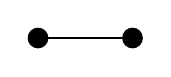
\begin{tikzpicture}
  \node[circle,fill=black,inner sep=2.5pt,draw] (a) at (180:0.6cm) {};
  \node[circle,fill=black,inner sep=2.5pt,draw] (b) at (0:0.6cm) {};
  \draw[thick] (a) -- (b);
\end{tikzpicture}

    \end{figure}
    \column<4->{0.14\textwidth}
    \centering
    \begin{figure}
      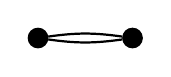
\begin{tikzpicture}
  \node[circle,fill=black,inner sep=2.5pt,draw] (a) at (180:0.6cm) {};
  \node[circle,fill=black,inner sep=2.5pt,draw] (b) at (0:0.6cm) {};
  \draw[thick] (a) edge[bend left=8] (b);
  \draw[thick] (a) edge[bend right=8] (b);
\end{tikzpicture}

    \end{figure}
    \column<5->{0.14\textwidth}
    \centering
    \begin{figure}
      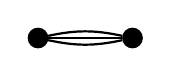
\begin{tikzpicture}
  \node[circle,fill=black,inner sep=2.5pt,draw] (a) at (180:0.6cm) {};
  \node[circle,fill=black,inner sep=2.5pt,draw] (b) at (0:0.6cm) {};
  \draw[thick] (a) edge[bend left=12] (b);
  \draw[thick] (a) edge[bend right=12] (b);
  \draw[thick] (a) -- (b);
\end{tikzpicture}

    \end{figure}
    \column<8->{0.14\textwidth}
    \centering
    \begin{figure}
      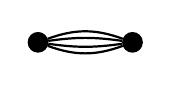
\begin{tikzpicture}
  \node[circle,fill=black,inner sep=2.5pt,draw] (a) at (180:0.6cm) {};
  \node[circle,fill=black,inner sep=2.5pt,draw] (b) at (0:0.6cm) {};
  \draw[thick] (a) edge[bend left=20] (b);
  \draw[thick] (a) edge[bend left=8] (b);
  \draw[thick] (a) edge[bend right=8] (b);
  \draw[thick] (a) edge[bend right=20] (b);
\end{tikzpicture}

    \end{figure}
  \end{columns}

  \begin{columns}[T]
    \column{0.1\textwidth}
    \column{0.40\textwidth}
    \centering 
    \visible<7->{
    	\begin{alertblock}{Not allowed!}
    	  Triangles are not possible sub-graphs in RBM
    	\end{alertblock}
    }
    \column<6->{0.14\textwidth}
    \centering
    \begin{figure}
      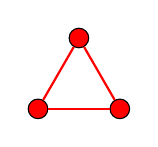
\begin{tikzpicture}
  \node[circle,fill=red,inner sep=2.5pt,draw] (a) at (90:0.6cm) {};
  \node[circle,fill=red,inner sep=2.5pt,draw] (b) at (210:0.6cm) {};
  \node[circle,fill=red,inner sep=2.5pt,draw] (c) at (330:0.6cm) {};
  \draw[red, thick] (a) -- (b);
  \draw[red, thick] (b) -- (c);
  \draw[red, thick] (c) -- (a);
\end{tikzpicture}

    \end{figure}
    \column<9->{0.14\textwidth}
    \centering
    \begin{figure}
      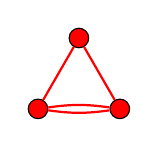
\begin{tikzpicture}
  \node[circle,fill=red,inner sep=2.5pt,draw] (a) at (90:0.6cm) {};
  \node[circle,fill=red,inner sep=2.5pt,draw] (b) at (210:0.6cm) {};
  \node[circle,fill=red,inner sep=2.5pt,draw] (c) at (330:0.6cm) {};
  
  \draw[red, thick] (a) -- (b);
  \draw[red, thick] (b) edge[bend left=8]  (c);
  \draw[red, thick] (b) edge[bend right=8] (c);
  \draw[red, thick] (c) -- (a);
\end{tikzpicture}
    \end{figure}
  \end{columns}

  \begin{columns}[T]
    \column{0.1\textwidth}
    \column{0.45\textwidth}
    \centering  
    \visible<11->{
    	\begin{alertblock}{Uncomputable}
      	They require \(O{(n^2m^2)}\) iterations to be computed
    	\end{alertblock}
    }
    \column{0.1\textwidth}
    \column<10->{0.14\textwidth}
    \centering
    \begin{figure}
      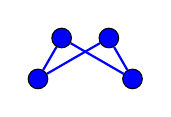
\begin{tikzpicture}
  \node[circle,fill=blue,inner sep=2.5pt,draw] (a) at (180:0.6cm) {};
  \node[circle,fill=blue,inner sep=2.5pt,draw] (b) at (0:0.6cm) {};
  \node[circle,fill=blue,inner sep=2.5pt,draw] (c) at (60:0.6cm) {};
  \node[circle,fill=blue,inner sep=2.5pt,draw] (d) at (120:0.6cm) {};

  \draw[blue, thick] (a) -- (c);
  \draw[blue, thick] (b) -- (c);
  \draw[blue, thick] (a) -- (d);
  \draw[blue, thick] (b) -- (d);
\end{tikzpicture}

    \end{figure}
  \end{columns}
\end{frame}

\begin{frame}
  \frametitle{Expression for \(\Gamma\)}
  Third order approximation of \(\Gam{\vec{m}^v, \vec{m}^h}{1}\) is
  \begin{align*}
    &\quad\sum_{i=1}^{m}\left[\log{\left(\mvi\right)}\mvi + \log{\left(1-\mvi\right)}(1-\mvi)-b_i\mvi\right]\\
    &+\sum_{j=1}^{n}\left[\log{\left(\mhj\right)}\mhj+\log{\left(1-\mhj\right)}(1-\mhj)-c_j\mhj\right]\\
    &-\sum_{i,j=1}^{m,n}\Bigg[
    \mvi w_{i,j}\mhj
    +\frac{1}{2}w_{i,j}^2\left(\mvi-\mvisq\right)\left(\mhj-\mhjsq\right)+\\
    &\qquad\quad+\frac{2}{3}w_{i,j}^3\left(\mvi-\mvisq\right)\left(\frac{1}{2}-\mvi\right)\left(\frac{1}{2}-\mhj\right)
    \left(\mhj-\mhjsq\right)\Bigg]
  \end{align*}
\end{frame}

\begin{frame}
  \frametitle{Minimization  of \(\Gamma\)}
  We have to find the minimum of \(\Gamma\)
  \[
  \left.\ParDer{\Gam{\vec{m}}{1}}{\vec{m}}\right|_{\vec{m}=\vec{\hat{m}}}=0.
  \]
  \pause
  We  have to solve these equations, we can do it iteratively
  \begin{align*}
    \hmvi&=\sigmoid{b_i + \sum_{j=1}^n\left[w_{i,j}\hmhj+
      \left(\hmhj-\hmhjsq\right)w^2_{i,j}\left(\frac{1}{2}-\hmvi\right)
      + \cdots \right]}\\
    \hmhj&=\sigmoid{c_j + \sum_{i=1}^m\left[w_{i,j}\hmvi+
      \left(\hmvi-\hmvisq\right)w^2_{i,j}\left(\frac{1}{2}-\hmhj\right)  + \cdots \right]}
  \end{align*}
	\pause
  \begin{columns}
    \begin{column}{0.7\textwidth}
      \begin{alertblock}{Multiple solutions!}
        Iterative procedure may lead to a local minimum (or even a maximum!)
      \end{alertblock}
    \end{column}
  \end{columns}
\end{frame}

\begin{frame}
  \frametitle{Computing the gradient of \(\FEn{\vec{0}}{1}\)}
  Recalling that
  \[
  \ParDer{\left(\FEn{\vec{0}}{1}\right)}{\vec{\theta}} =
  \ParDer{\left(\Gam{\vec{\hat{m}}}{1}\right)}{\vec{\theta}}
  \]  
  We  have these expressions for the  likelihood gradient
  \begin{align*}
    \ParDer{\left(\Gam{\vec{\hat{m}}}{1}\right)}{b_i} &= -\hmvi\\
    \ParDer{\left(\Gam{\vec{\hat{m}}}{1}\right)}{c_j} &= -\hmhj\\
    %
    \ParDer{\left(\Gam{\vec{\hat{m}}}{1}\right)}{w_{i,j}}
    &=-\Bigg[\hmvi\hmhj +w_{i,j}\left(\hmvi-\hmvisq\right)\left(\hmhj-\hmhjsq\right)+ \cdots \Bigg]
  \end{align*}
\end{frame}

%%%%%%%%%%%%%%%%%%%%%%%%%%%%%%%%%%%%%%%%%%%%%%%%%%%%%%%%%%%%%%%%%%%%%%%%%%%%%%%%%%%%%%%%%%%%%%%%%%%%

\subsection{Algorithm}
\begin{frame}
  \frametitle{The algorithm}
  Once per batch:
  \begin{enumerate}
    \item Pick \(\ell\) magnetizations \(\{\vec{m}_k\}_{k=1,\dots,\ell}\) randomly.
    \item Apply consistency equations \(k\) times to converge to \(\{\vec{\hat{m}}_k\}_{k=1,\dots,\ell}\)
    \item Compute \(\FEn{\vec{0}}{1}\) gradient for each \(\vec{\hat{m}}_k\)
    \item Average the gradient using \(e^{-\Gam{\vec{\hat{m}}_k}{1}}\) as weights
  \end{enumerate}
	\pause
  \(\ell\) and \(k\) are additional meta-parameters of the algorithm.\\
  \pause
  The \alert{weight decay} plays a fundamental role in keeping  the hypothesis of high temperature satisfied
  \pause
  \begin{columns}
   \column{0.8\textwidth}
     \begin{alertblock}{Persistent EMF}
       As for contrastive divergence, we can implement a \emph{persistent} version, where magnetizations are stored among different batches
     \end{alertblock}
  \end{columns}
\end{frame}


















